\documentclass{fkssolpub}

\usepackage[czech]{babel}
\usepackage{fontspec}
\usepackage{fkssugar}
\usepackage{amsmath}
\usepackage{graphicx}

\author{Ondřej Sedláček}
\school{Gymnázium Oty Pavla} 
\series{1}
\problem{2} 

\begin{document}

\begin{figure}
	\begin{center}
		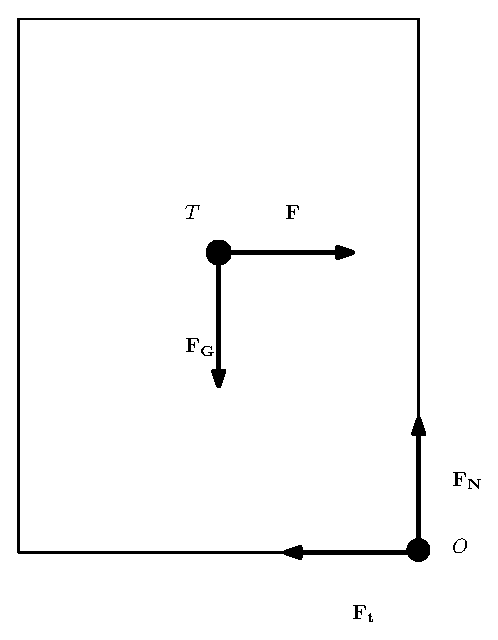
\includegraphics[width=0.5\textwidth]{2-fig.eps}
	\end{center}
	\caption{Náčrtek sil působících na těleso.}
	\label{fig:1}
\end{figure}

Víme, že na filodendron bude v okamžiku, kdy jsou ještě síly v rovnováze a nezpůsobí převržení květináče, působit síly načrtnuté na obrázku. Z rovnováhy sil pak víme, že platí:

\[
	F_g = F_N
\]
\[
	F_t = F
\]

A z rovnováhy momentů sil v bodě $O$ víme, že platí:

\[
	F h = F_G r
\]

kde $h$ je výška těžistě a $r$ je poloměr podstavy.

Z této rovnice nakonec jsme schopni zjistit maximální velikost síly $F$ a tím pádem i maximální zrychlení květináče:

\[
	F h = F_G r
\]
\[
	F = \frac{F_G r}{h}
\]
\[
	a = \frac{g r}{h} = \frac{6}{7} g
\]

Při zatáčení bude na květináč působit dostředivé zrychlení, které může být maximálně $a$. Proto maximální rychlost při projíždění zatáčky $v_z$ je:

\[
	a = \frac{v_z^2}{R} = \frac{6}{7} g
\]
\[
	v_z = \sqrt{\frac{6}{7} g R} \doteq "9{,}17 m \cdot s^{-1}"
\]

Brždění tedy bude trvat:

\[
	t = \frac{v - v_z}{a}
\]

A při brždění ujede:

\[
	s = v t - \frac{1}{2} a t^2 = v \frac{v - v_z}{a} - \frac{(v - v_z)^2}{2a} = \frac{v - v_z}{a} \left(v - \frac{v - v_z}{2} \right) = \frac{v^2 - v_z^2}{2a} = "32{,}16 m"
\]

Tedy musí začít brzdit alespoň tolik metrů před tím, než vjede do zatáčky.



\end{document}
